\documentclass[11pt,a4paper]{article}
%%%%%%%%%%%%%%%%%%
% pandoc command %
%%%%%%%%%%%%%%%%%%

%pandoc --bibliography=references.bib --bibliography=references_local.bib -o main.docx main.tex --citeproc --csl=SBL.csl
%I took the .csl file directly from zotero -> modify style -> save as...


\usepackage{hyphenat}
\usepackage{tabularx}
\usepackage{hyperref}
\usepackage{makecell}
\usepackage[utf8]{inputenc}
\usepackage{tipa} %phonetic characters
\usepackage{lua-ul} %pour barrer du texte avec la commande \strikeThrough
\usepackage[autostyle]{csquotes}
\MakeOuterQuote{"}

\usepackage[document]{ragged2e} %Permet de régler les alignements
\let\oldfootnote\footnote
\renewcommand{\footnote}[1]{\oldfootnote{\justifying #1}} %Justify footnotes

\usepackage[dvipsnames]{xcolor} %Allow colors

% -------------------------------
%  Language Hebrew & Greek     
% -------------------------------
\usepackage{polyglossia} %[babelshorthands] permet d'avoir les guillemets allemands avec le code "`toto"' et les guillemets français avec le code "<tata">
\setdefaultlanguage[variant=american]{english}
%\PolyglossiaSetup{english}{indentfirst=false}
\setotherlanguages{french, hebrew, syriac, greek}
\hyphenation{manu-script, manu-scripts, stem-ma, inter-relation-ship}
% ------------------------
% Define fonts
% ------------------------

\usepackage{fontspec}
\setmainfont[]{cochineal}
% %\setmainfont[Path=./fonts/,
%  BoldFont={Brill-Bold.ttf}, 
%  ItalicFont={Brill-Italic.ttf},
%  BoldItalicFont={Brill-BoldItalic.ttf}
%  ]{Brill-Roman.ttf}
 
\newfontfamily{\hebrewfont}[Script=Hebrew, Path=./fonts/]{SBL_Hbrw.ttf}
\newfontfamily{\hebrewfontsf}[Script=Hebrew]{Miriam CLM}
\newfontfamily{\hebrewfonttt}[Script=Hebrew]{Miriam Mono CLM}
%\newfontfamily\hebrewfont[Script=Hebrew]{SBL_BLit.ttf}
\newfontfamily\syriacfont[Script=Syriac, Path=./fonts/]{EstrangeloEdessa.ttf}



% ---------------------------
% Image Package
% ---------------------------
\usepackage{graphicx}
\usepackage{pdfpages}
\graphicspath{ {./img/} }
\usepackage{float} %Pour placer les figures au bon endroit
% ---------------------------



% ---------------------------
% Define Bibliography
% ---------------------------
% Load main style
% Pass indexing=cite to biblatex (if you want author indexing)
\PassOptionsToPackage{indexing=cite}{biblatex}
% Pass jblstyle to sbl-paper if you want double spaced footnotes
% \usepackage{sbl-paper}
%\usepackage[style=sbl,doi=false,issn=false,isbn=false,url=false,eprint=false,]{biblatex}
\usepackage[style=sbl]{biblatex}


\DeclareSourcemap{
  \maps[datatype=bibtex]{
    \map{
      \step[fieldset=doi, null]
      \step[fieldset=language, null]
      \step[fieldset=issn, null]{}
      \step[fieldset=url, null]{}
      \step[fieldset=isbn, null]{}
      \step[fieldset=eprint, null]{}
    }
  }
}

%doi=false,issn=false,isbn=false,url=false,eprint=false,

% Add your bib resource here

\addbibresource{references.bib}
\addbibresource{references_local.bib}
%\addbibresource{biblio.bib}
\useshorttitle
\AtEveryBibitem{\clearlist{language}\clearfield{doi}}



%%%%%%%%%%%%%%%%%%%
% Create todolist %
%%%%%%%%%%%%%%%%%%%

\usepackage{enumitem,amssymb}
\newlist{todolist}{itemize}{2}
\setlist[todolist]{label=$\square$}


% ---------------------------------------------------------------------

\usepackage{pdfpages}
\usepackage{geometry}
 \geometry{
 a4paper,
 left=25mm,
 right=15mm,
 top=15mm,
 }

 
\title{Introduction à la critique textuelle\\Critique textuelle de la bible hébraïque}
\author{Frédérique Michèle Rey, Sophie Robert-Hayek}
\date{September 2024}

\begin{document}

\maketitle
\justifying

\section{La \textit{Biblia Hebraica Stuttgartensia} \& La \textit{biblia Hebraica Quinta}}

\subsection{Comparaison BHS - Codex Leningrad}
\begin{figure}[!h]
    \centering
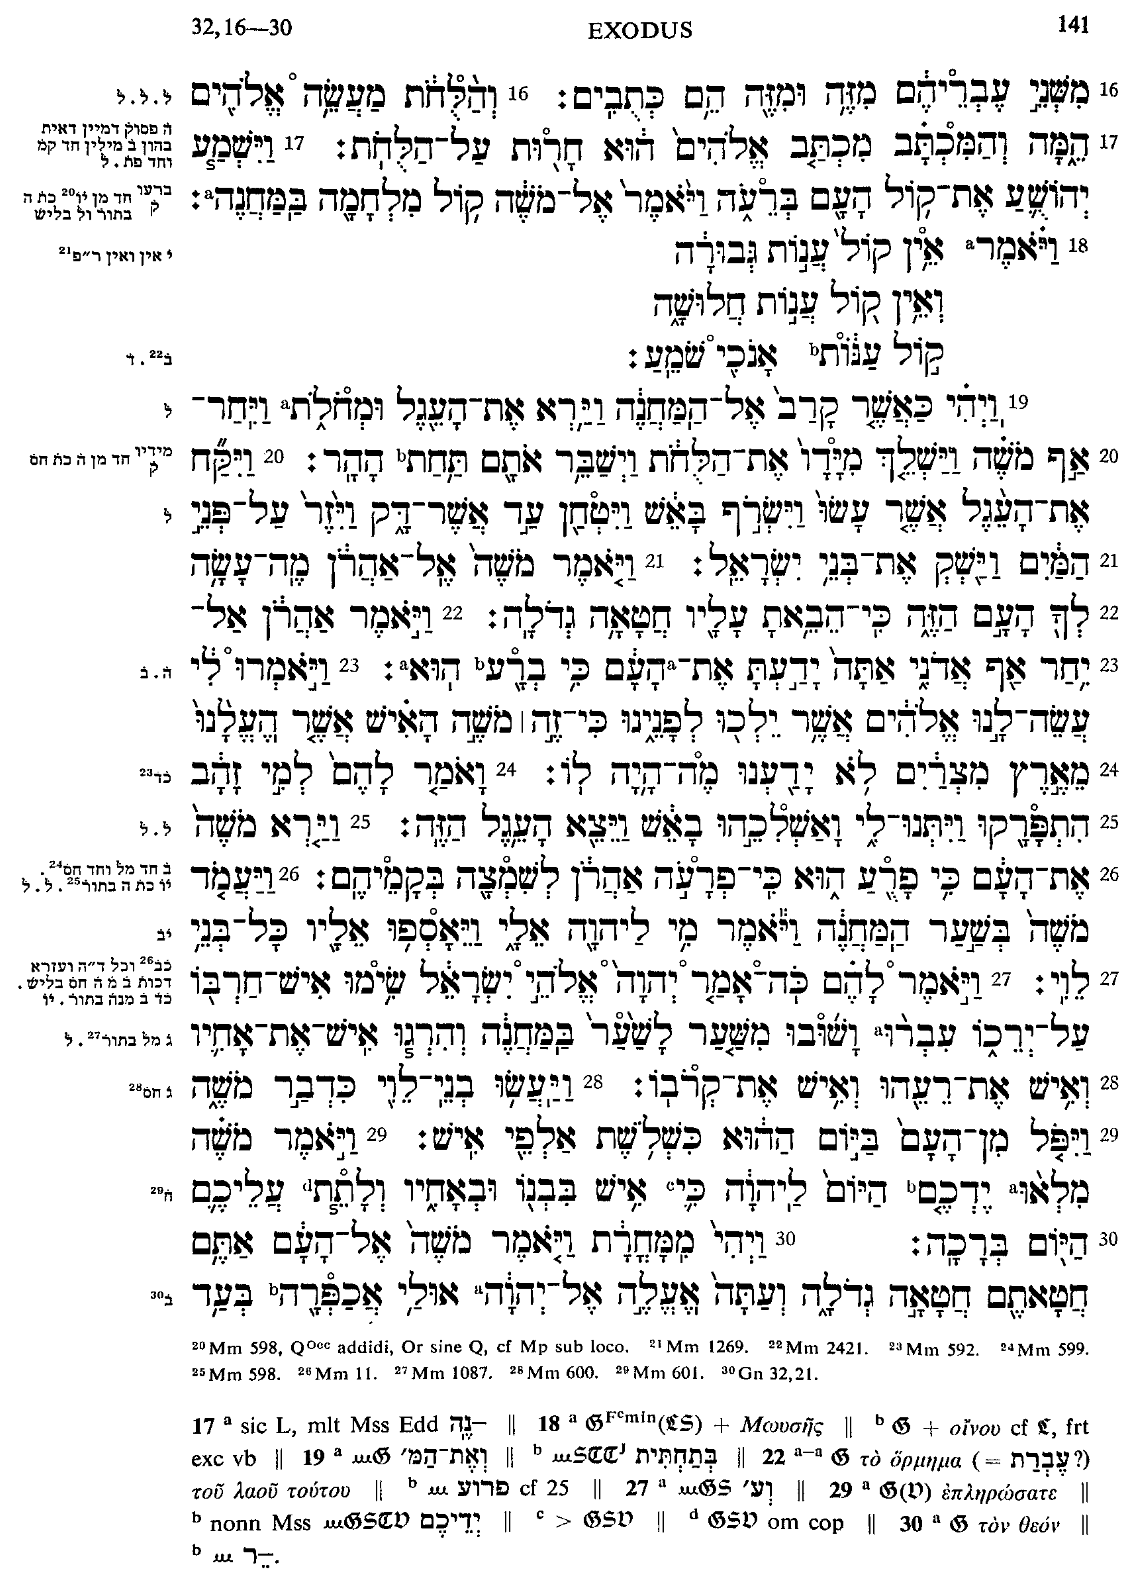
\includegraphics[width=.6\linewidth]{img/BHS_Exod_32.png}
\end{figure}
\newpage
\begin{figure}[!h]
    \centering
\includegraphics[width=1\linewidth]{img/Leningrad_Exod_32.jpg}
\end{figure}

% \begin{figure}[h]
%     \begin{minipage}[c]{.46\linewidth}
%         \centering            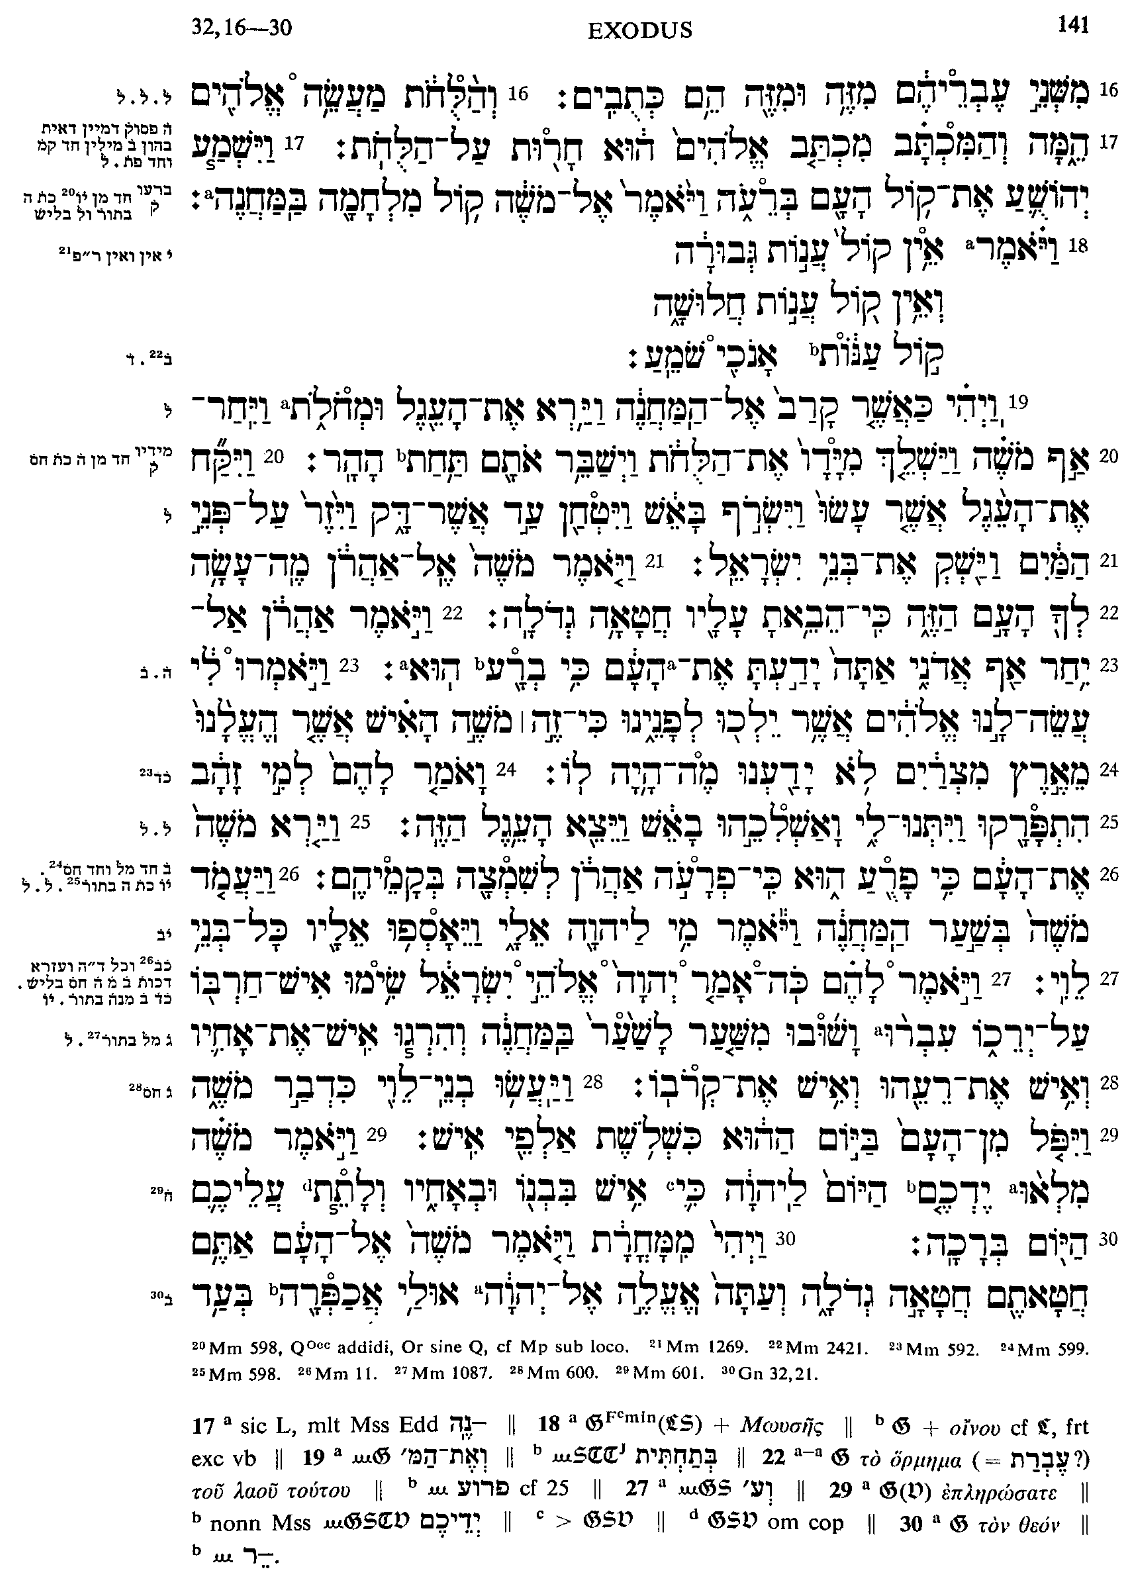
\includegraphics[width=1\linewidth]{img/BHS_Exod_32.png}
%     \end{minipage}
%     \hfill%
%     \begin{minipage}[c]{.46\linewidth}
%         \centering
%         \includegraphics[width=1\linewidth]{img/Leningrad_Exod_32.jpg}
%     \end{minipage}
% \end{figure}
\newpage

\subsection{Lire un apparat critique, Ruth 1,1}
\begin{figure}[!h]
    \centering
    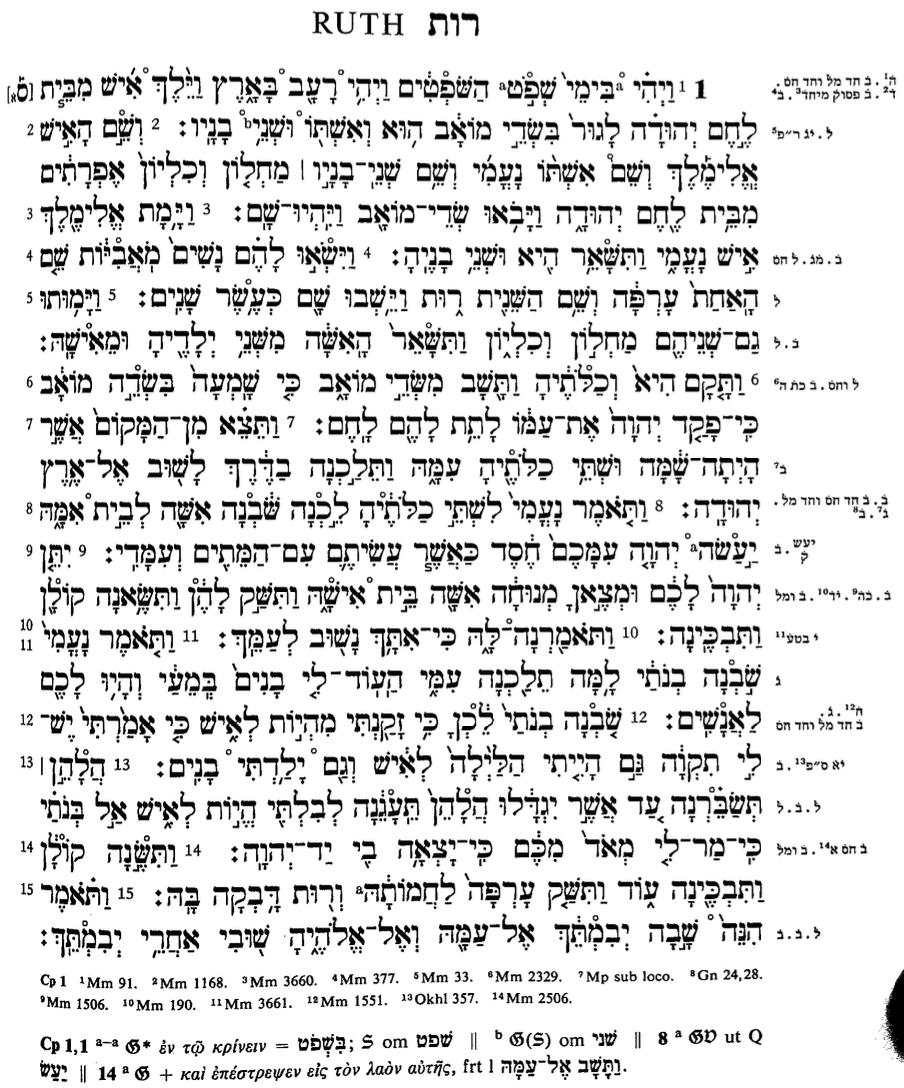
\includegraphics[width=.8\linewidth]{img/Ruth_1_1.png}
\end{figure}
\textbf{Questions:}
    \begin{itemize}
        \item Quel est le texte édité ?
        \item Quelle sont les différentes zone autour du texte ?
        \item Identifier les deux premiers lieux variants et expliquer l'apparat critique.
        \item Vérifier votre propre réponse à la question précédente en allant consulter (en ligne) les témoins et/ou les éditions concernées.
    \end{itemize}
\newpage
\subsection{Construire un apparat critique : Ruth 1--2}
\paragraph{Textes}~\\

\textbf{Codex de Leningrad}\\
\texthebrew{
\textfrench{1}
וַיְהִ֗י בִּימֵי֙ שְׁפֹ֣ט הַשֹּׁפְטִ֔ים וַיְהִ֥י רָעָ֖ב בָּאָ֑רֶץ וַיֵּ֨לֶךְ אִ֜ישׁ מִבֵּ֧ית לֶ֣חֶם יְהוּדָ֗ה לָגוּר֙ בִּשְׂדֵ֣י מוֹאָ֔ב ה֥וּא וְאִשְׁתּ֖וֹ וּשְׁנֵ֥י בָנָֽיו׃\\
%\RTL\noindent
\textfrench{2}
וְשֵׁ֣ם הָאִ֣ישׁ אֱ‍ֽלִימֶ֡לֶךְ וְשֵׁם֩ אִשְׁתּ֨וֹ נָעֳמִ֜י וְשֵׁ֥ם שְׁנֵֽי־ בָנָ֣יו ׀ מַחְל֤וֹן וְכִלְיוֹן֙ אֶפְרָתִ֔ים מִבֵּ֥ית לֶ֖חֶם יְהוּדָ֑ה וַיָּבֹ֥אוּ שְׂדֵי־ מוֹאָ֖ב וַיִּֽהְיוּ־ שָֽׁם׃\\}


\textbf{4Q104 (4QRuth${^a}$) frg. 1, lignes 1--4}\\
\texthebrew{
\textfrench{1}
 ויהי בימי שפט השפטים ויהי רעב בארץ וילך איש מ[בית לחם]\\
\textfrench{2}
יהודה לגור בשדה מואב הוא ואשתו ושני בניו ושם האי[ש אלימלך]\\
\textfrench{3}
ושם אשתו נעמי ושם שני בניו מחלון וכליון אפרתים מ֯[בית לחם]\\
\textfrench{4}
 [יהו]דה ויבאו שדה מואב וישבו שם\\
 }

\textbf{4Q105 (4QRuth${^b}$) frg. 1-3, lignes 1--2}\\

\texthebrew{
\textfrench{1}
בניו  ש[ם~~~~~~~~~~~~~~~~~~~~~~~~~~~~~~~~~~~~~]\\
\textfrench{2}
מבית לח֯[ם~~~~~~~~~~~~~]ש֯די[~~~~~~~~~~~~~~~~~~~~]\\
}

\textbf{Codex Alexandrinus}\\
1 \textgreek{Καὶ ἐγένετο ἐν ταις ημεραις εν τῷ κρίνειν τοὺς κριτὰς καὶ ἐγένετο λιμὸς ἐν τῇ γῇ, καὶ ἐπορεύθη ἀνὴρ ἀπὸ Βαιθλεεμ τῆς Ιουδα τοῦ παροικῆσαι ἐν ἀγρῷ Μωαβ, αὐτὸς καὶ ἡ γυνὴ αὐτοῦ καὶ οἱ δυο υἱοὶ αὐτοῦ.}\\
2 \textgreek{καὶ ὄνομα τῷ ἀνδρὶ Αβιμελεχ, καὶ ὄνομα τῇ γυναικὶ αὐτοῦ Νωεμιν, καὶ ὄνομα τοῖς δυσὶν υἱοῖς αὐτοῦ Μααλων καὶ Χελαιων, Εφραθαῖοι ἐκ Βαιθλεεμ τῆς Ιουδα· καὶ ἤλθοσαν εἰς ἀγρὸν Μωαβ καὶ ἦσαν ἐκεῖ.}\\
    
% \textbf{Peshitta}\\
% \textsyriac{
% \textfrench{1}
% ܘܗܼܘܐ ܒܝܘ̈ܡܝ ܕܝܿܢ̈ܐ܀ ܗܼܘܐ ܟܦܢܐ ܒܐܪܥܐ܂ ܘܐܙܠ ܓܒܪܐ ܡܢ ܒܝܬ ܠܚܡ ܕܝܗܘܕܐ ܠܡܥܡܪ ܒܐܪܥܐ ܕܡܘܐܒ܃ ܗܼܘ ܘܐܢܬܬܼܗ ܘܒ̈ܢܘܗܝ ܡܛܠ ܕܥܼܫܢ ܟܦܢܐ ܒܐܪܥܐ܀\\
% \textfrench{2}
% ܘܫܡܗ ܠܓܒܪܐ ܐܠܝܡܠܟ܃ ܘܫܡܗܿ ܕܐܢܬܬܗ ܢܥܡܝ܂ ܘܫܡܗ̈ܐ ܕܒܢܘ̈ܗܝ ܡܠܝܘܢ ܘܟܠܝܘܢ ܐܦܪ̈ܬܝܐ ܡܢ ܒܝܬ ܠܚܡ ܕܝܗܘܕܐ܂ ܘܐܬܘ ܠܐܪܥܐ ܕܡܘܐܒ ܠܡܥܡܪ ܬܡܢ܀\\}

Sur la base des témoins ci-dessus, refaire l'apparat critique de Ruth 1:1 et construire l'apparat critique de Ruth 1:2.\\
\begin{enumerate}
    \item Collation des manuscrits hébreux : aligner l'ensemble des témoins hébreux
    \item Collation des deux témoins grecs
   % \item \textbf{Bonus} Collation du texte  Syriaque
    \item \textbf{Bonus} chercher les témoins manuscrits sur Internet et vérifier les lectures données sur les photos des manuscrits.
\end{enumerate}

\section{Exercices étiologie de la variante}

\subsection{Exercice 1 – Jg 20:13}
TM: \texthebrew{וְלֹ֤א אָבוּ֙ בִּנְיָמִ֔ן} \\
\texthebrew{אָבוּ} Qal acc. 3ème pers. plur. \texthebrew{אבה} «vouloir» \\
«Ils ne voulurent pas Benjamin» \\
LXX: \textgreek{καὶ οὐκ εὐδόκησαν οἱ υἱοὶ Βενιαμιν} \\
\textbf{εὐδόκησαν} – Aor. 3ème pers. plur. de \textgreek{εὐδοκέω} «vouloir» \\
«Les fils de Benjamin ne voulurent pas»

\subsection{Exercice 2 – Dt 31:1}
TM: \texthebrew{וַיֵּ֖לֶךְ מֹשֶׁ֑ה וַיְדַבֵּ֛ר אֶת־הַדְּבָרִ֥ים הָאֵ֖לֶּה} \\
4QDeut${^b}$: \texthebrew{וַיְכַל משה לְדַבֵּר את כל הד[ברים} \\
\texthebrew{וַיְכַל} verbe inac. 3ème pers. masc. sing. de \texthebrew{כלה} «finir achever» \\
LXX: \textgreek{καὶ συνετέλεσεν Μωυσῆς λαλῶν πάντας τοὺς λόγους τούτους} \\
\textgreek{συνετέλεσεν} - aor. 3 pers. sing. de \textgreek{συντελέω} «finir» \\
\textgreek{λαλῶν} - \textgreek{λαλέω} part. pres. nom. masc. sing.

\subsection{Exercice 3 – Os 6:5}
TM: \texthebrew{וּמִשְׁפָּטֶ֖יךָ אֹ֥ור יֵצֵֽא} \\
\texthebrew{וּמִשְׁפָּטֶ֖יךָ} - Plur. + suf. 2ème pers. masc. sing. de \texthebrew{מִשְׁפָּט} «tes jugements» \\
LXX: \textgreek{καὶ τὸ κρίμα μου ὡς φῶς ἐξελεύσεται} \\
\textbf{ἐξελεύσεται} - \textgreek{ἐξέρχομαι} ind. fut. moyen 3ème pers. sing. «sortir»

\subsection{Exercice 4 – Psa 22:30}
TM: \texthebrew{וְ֝נַפְשֹׁ֗ו לֹ֣א חִיָּֽה} \\
\texthebrew{חִיָּֽה} Piel acc. 3 pers. masc. sing. de \texthebrew{חיה} «vivre» \\
LXX: \textgreek{καὶ ἡ ψυχή μου αὐτῷ ζῇ} \\
\textgreek{ζῇ} ind. prés. act. 3 pers. sing. de \textgreek{ζάω} "vivre"

\subsection*{Exercice 5 – Dt 32:8}
TM: \texthebrew{יַצֵּב֙ גְּבֻלֹ֣ת עַמִּ֔ים לְמִסְפַּ֖ר בְּנֵ֥י יִשְׂרָאֵֽל} \\
\texthebrew{יצב} Verbe Hiph. 3 masc. sing. de \texthebrew{נצב} «placer établir définir» \\
\texthebrew{גְּבֻלֹ֣ת} «frontières» \\
\texthebrew{מִסְפַּ֖ר} «nombre» \\
4QDeut${^j}$: \texthebrew{בני אלוהים} \\
LXX: \textgreek{ἔστησεν ὅρια ἐθνῶν κατὰ ἀριθμὸν ἀγγέλων θεοῦ} \\
\textbf{ἔστησεν} - \textgreek{ἵστημι} ind. aor. 3ème pers. sing. «établir placer» \\
\textbf{ὅρια} - acc. neutre plur. de \textgreek{ὅριον} «territoire» \\
Les manuscrits de la LXX varient entre \textgreek{ἀγγέλων θεοῦ} et \textgreek{υἱῶν θεοῦ} (voir l’apparat critique de la LXX)

\subsection*{Exercice 6 – Si 41:5}
Ms A: \texthebrew{שׁוֹמֵעַ לִי יִשׁפוֹט אֶמֶת} \\
«Celui qui m’écoute jugera (en) vérité» \\
LXX: \textgreek{ὁ ὑπακούων αὐτῆς κρινεῖ ἔθνη} \\
«Celui qui m’écoute jugera les nations» \\
\textbf{ὑπακούων} - part. prés. de \textgreek{ὑπακούω} «écouter»

\subsection*{Exercice 7 – Gn 15:11}
TM: \texthebrew{וַיַּשֵּׁ֥ב אֹתָ֖ם אַבְרָֽם} \\
\texthebrew{וַיַּשֵּׁ֥ב} - Hiph. 3 pers. masc. sing. de \texthebrew{נשב} «chasser renvoyer» \\
LXX: \textgreek{καὶ συνεκάθισεν αὐτοῖς Αβραμ} \\
\textbf{συνεκάθισεν} - ind. aor. 3 pers. sing. \textgreek{συγκαθίζω} «s’assoir avec» \\

\newpage
\section{Travaux pratiques - Analyse de Deut 32}
\subsection{Texte et traduction de 4Q44}
\begin{figure}[!h]
    \begin{minipage}[c]{.46\linewidth}
        \centering`
        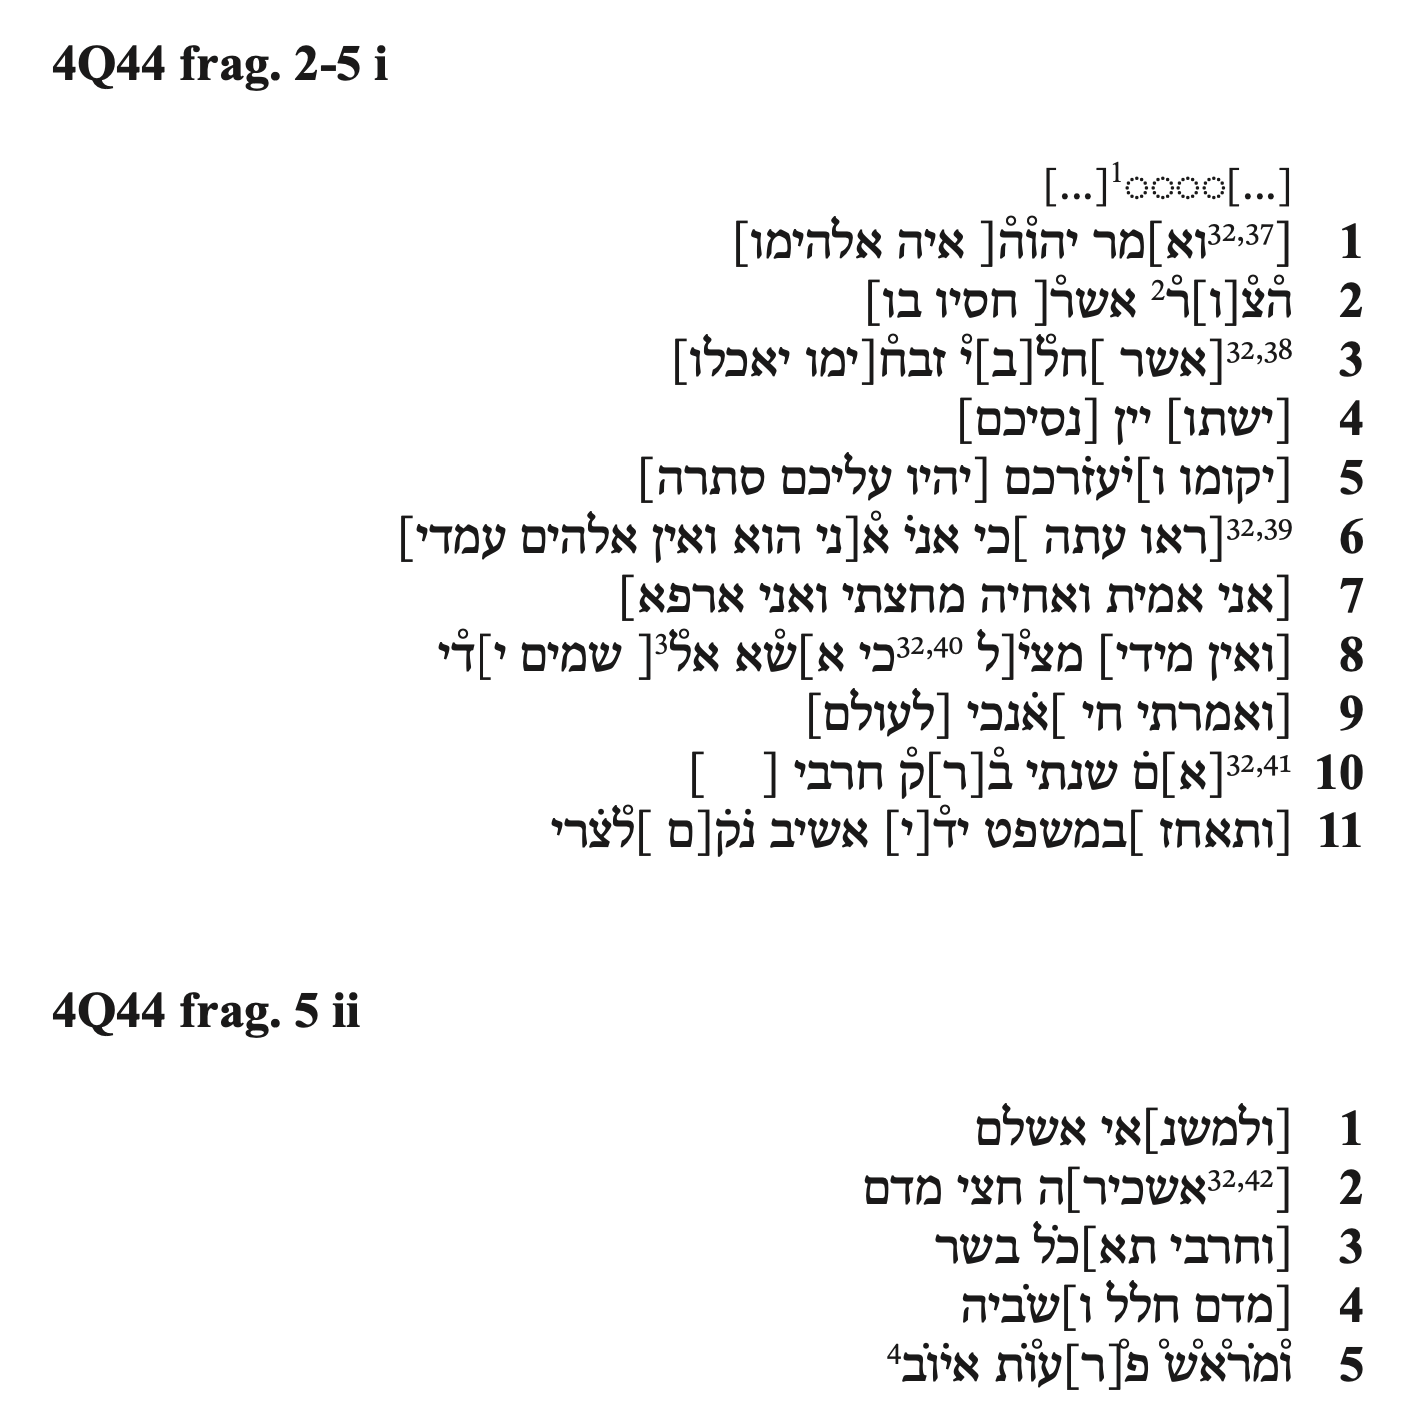
\includegraphics[width=1\linewidth]{img/4Q44/4Q44_1.png}
    \end{minipage}
    \hfill%
    \begin{minipage}[c]{.46\linewidth}
        \centering
        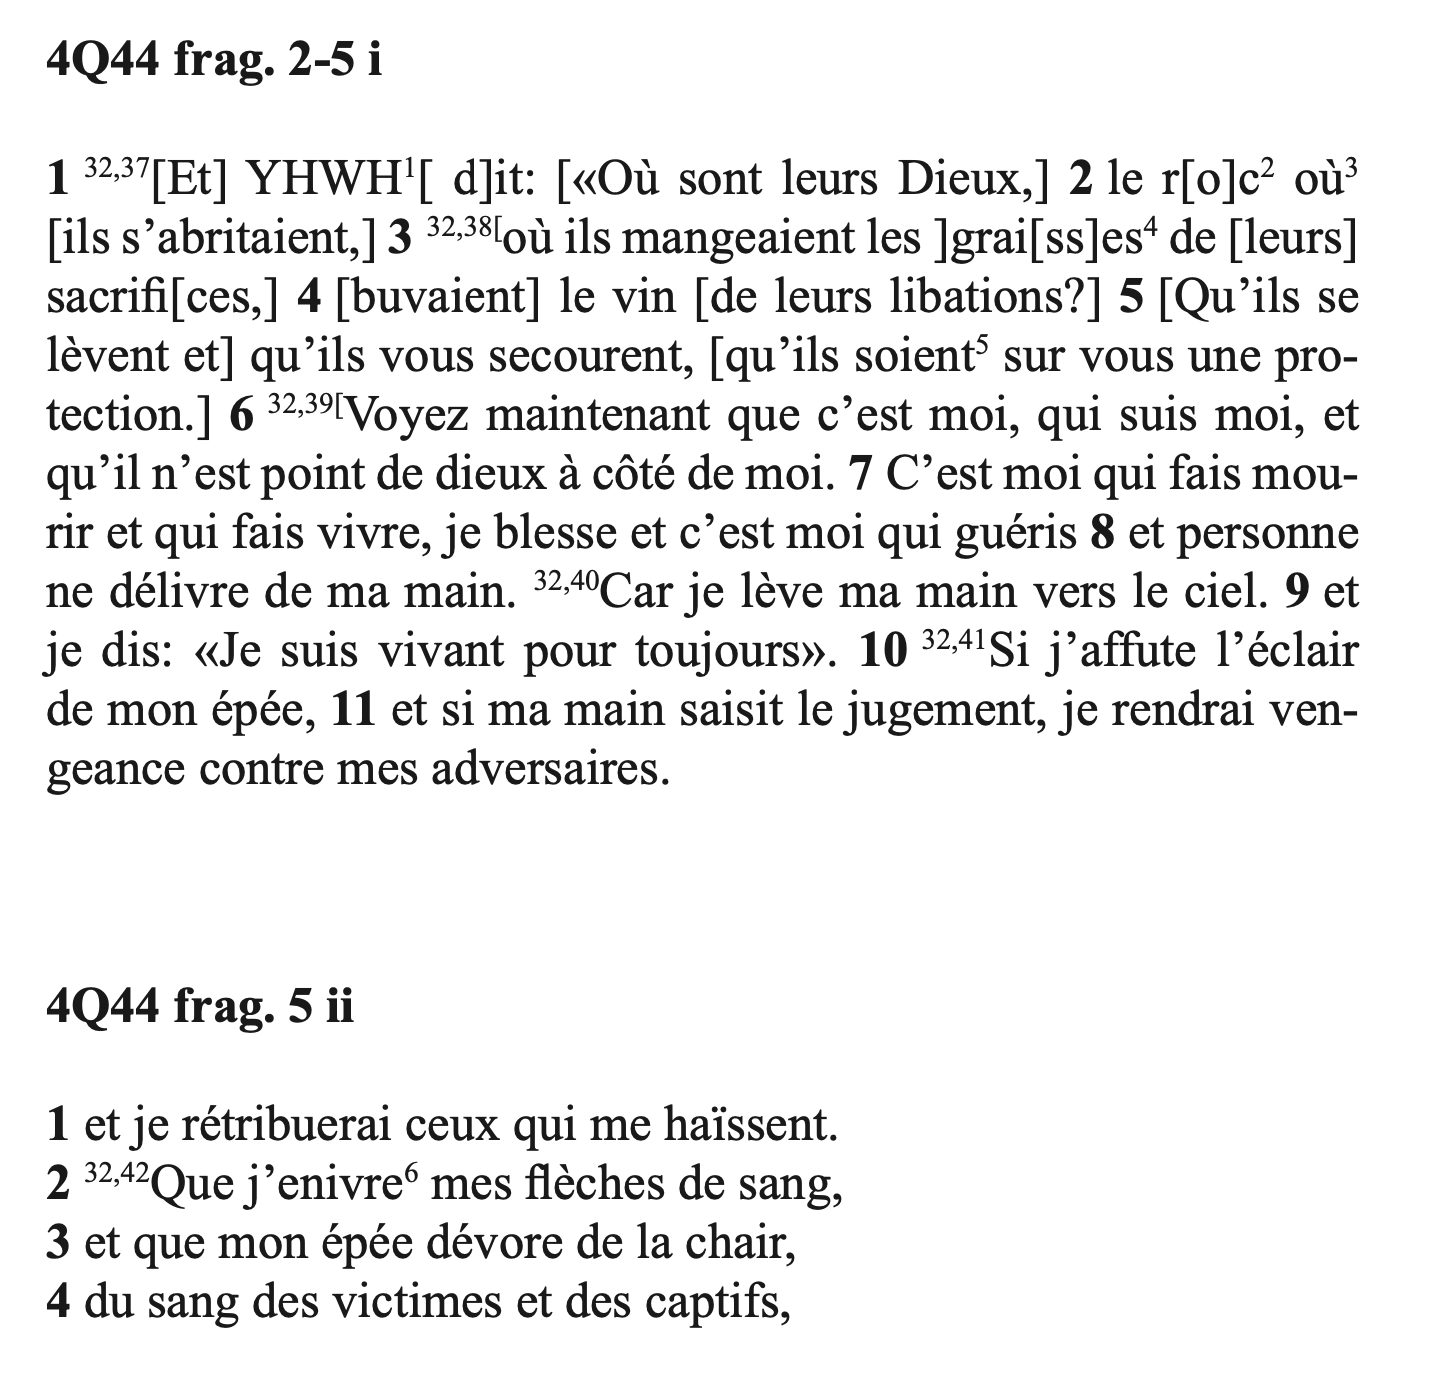
\includegraphics[width=1\linewidth]{img/4Q44/4Q44_trans_1.png}
    \end{minipage}
\end{figure}
\begin{figure}[!h]
    \begin{minipage}[c]{.46\linewidth}
        \centering`
        
\includegraphics[width=1\linewidth]{img/4Q44/4Q44_2.png}
    \end{minipage}
    \hfill%
    \begin{minipage}[c]{.46\linewidth}
        \centering
        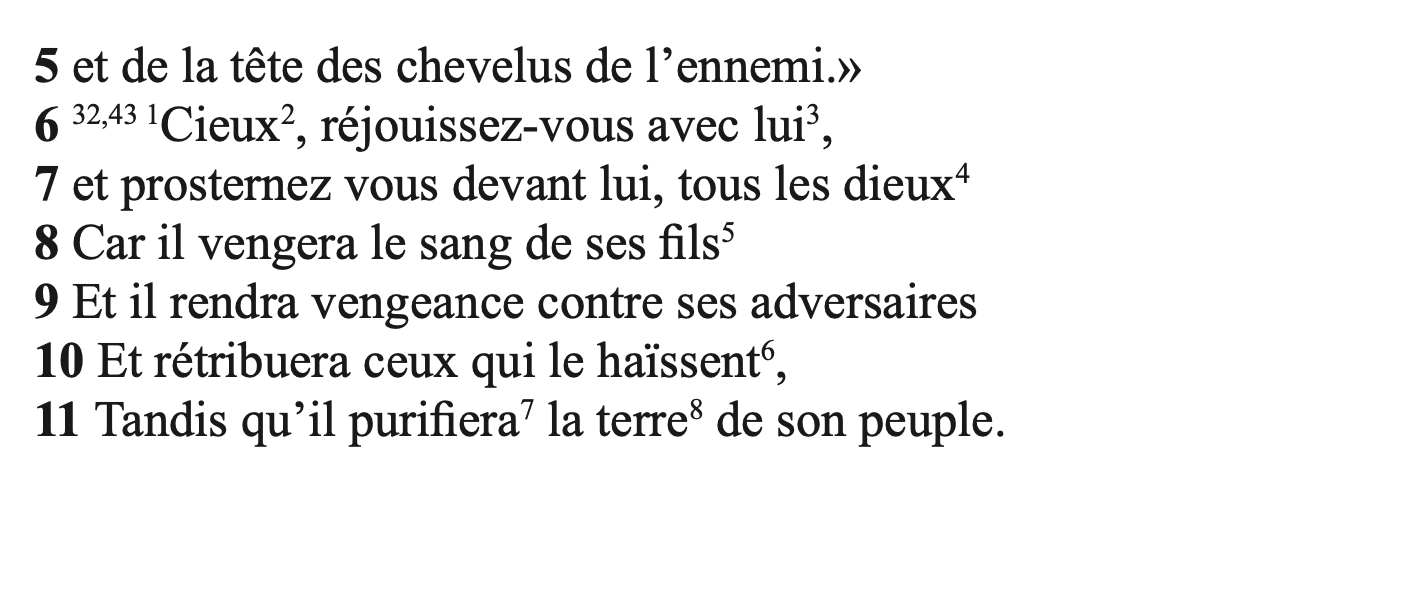
\includegraphics[width=1\linewidth]{img/4Q44/4Q44_trans_2.png}
    \end{minipage}
\end{figure}
\newpage
\subsection{Texte Massorétique}
\begin{figure}[!h]
    \begin{minipage}[c]{.46\linewidth}
        \centering`
        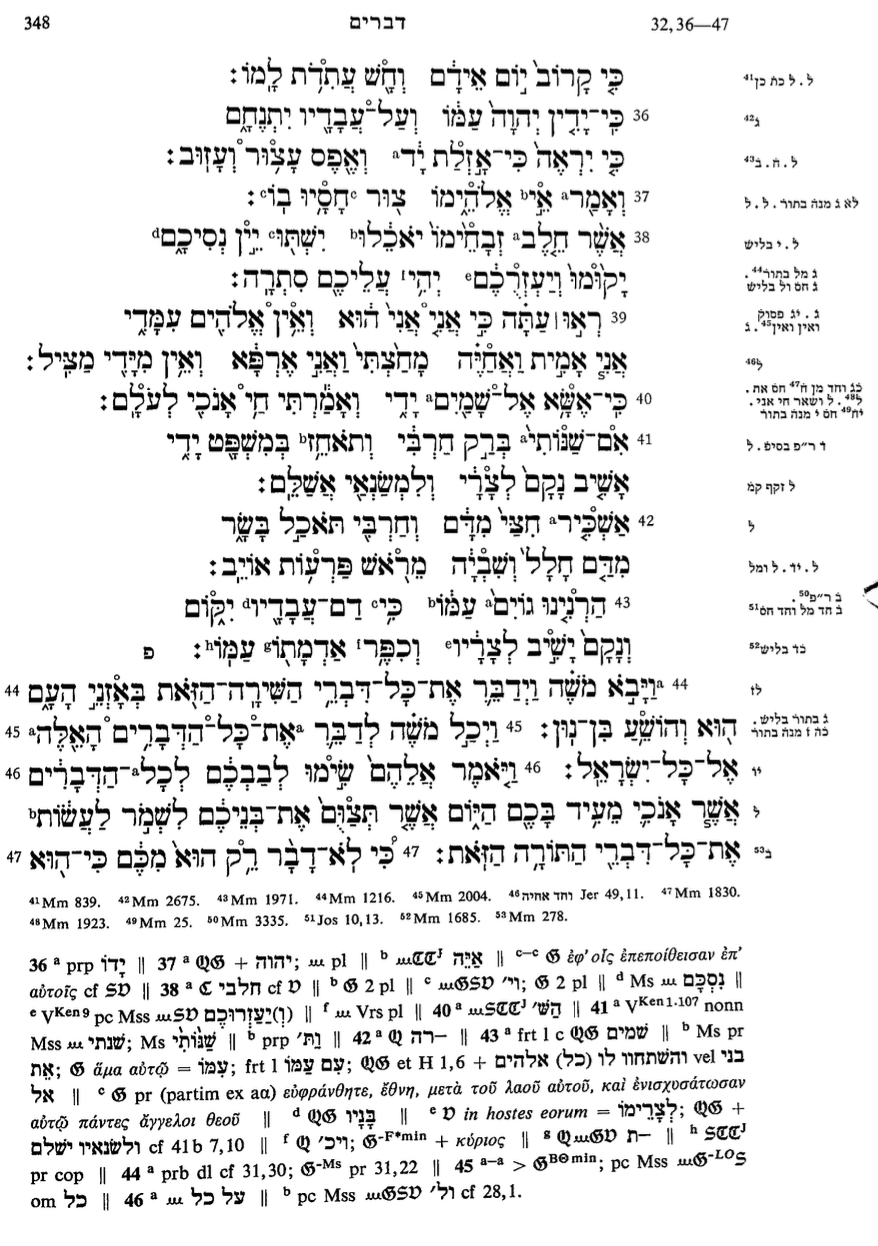
\includegraphics[width=1\linewidth]{img/4Q44/BHS_Dt_32_2.png}
    \end{minipage}
    \hfill%
    \begin{minipage}[c]{.46\linewidth}
        \centering
        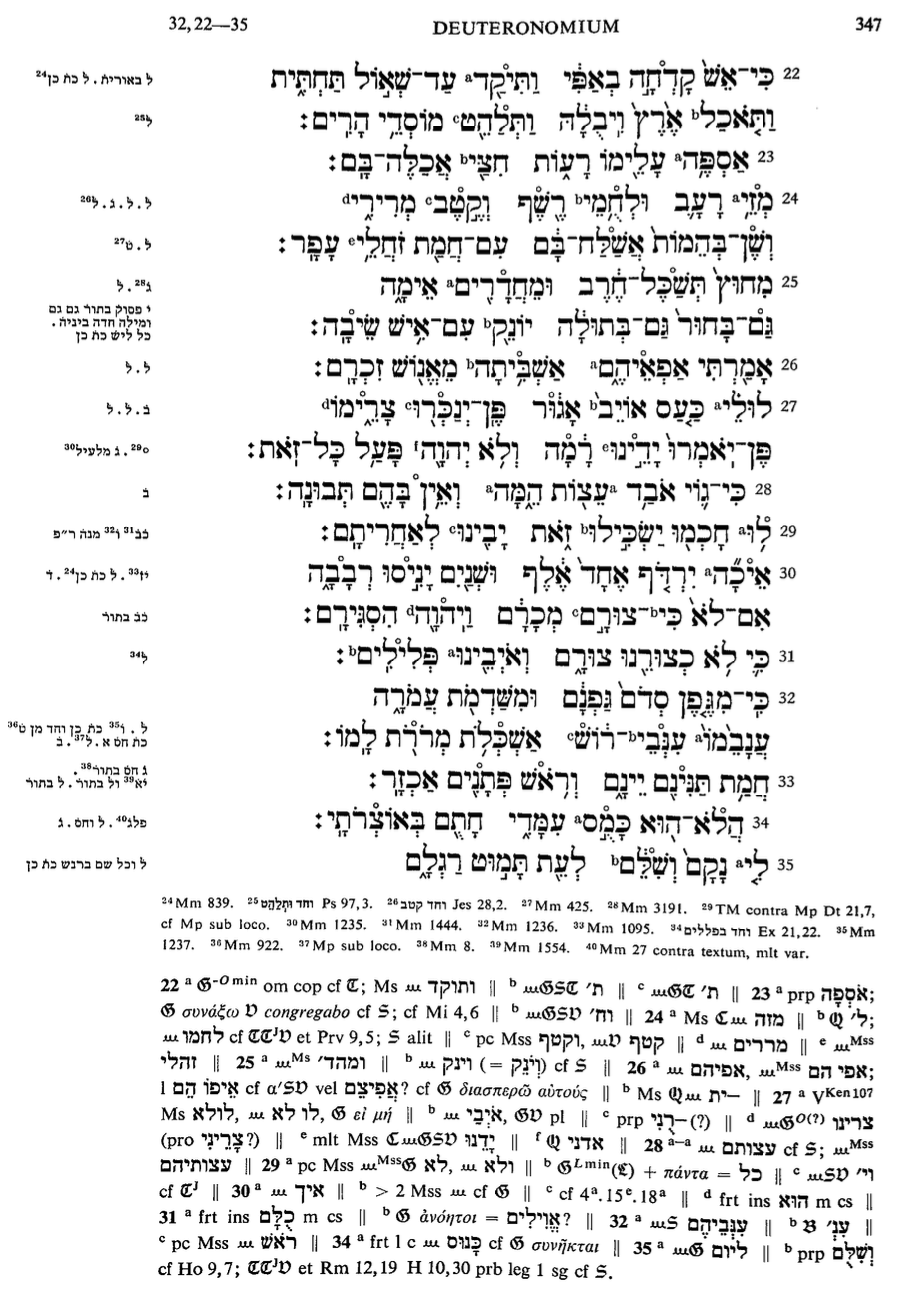
\includegraphics[width=1\linewidth]{img/4Q44/BHS_Dt_32_1.png}
    \end{minipage}
\end{figure}
\subsection{LXX}
\newpage
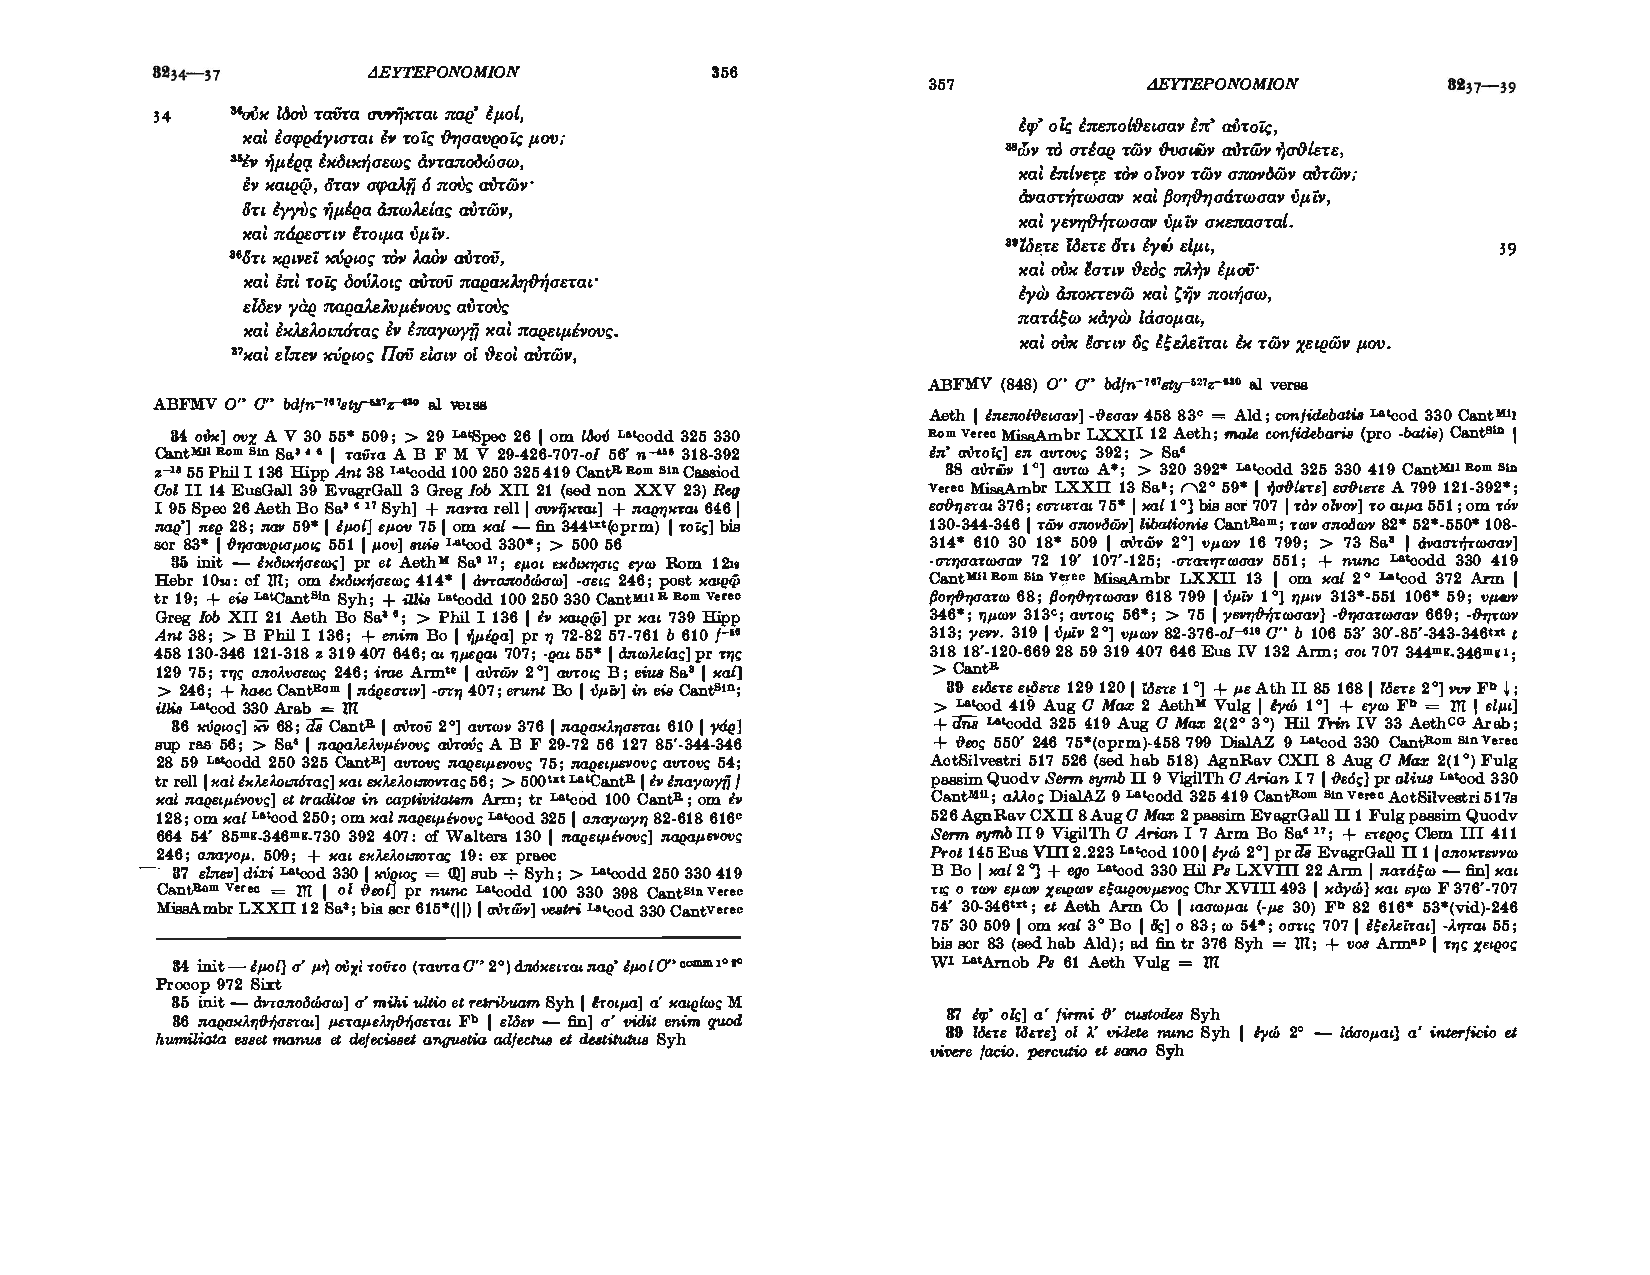
\includepdf[pages=1-2, angle=90]{img/4Q44/LXX.pdf}
\newpage
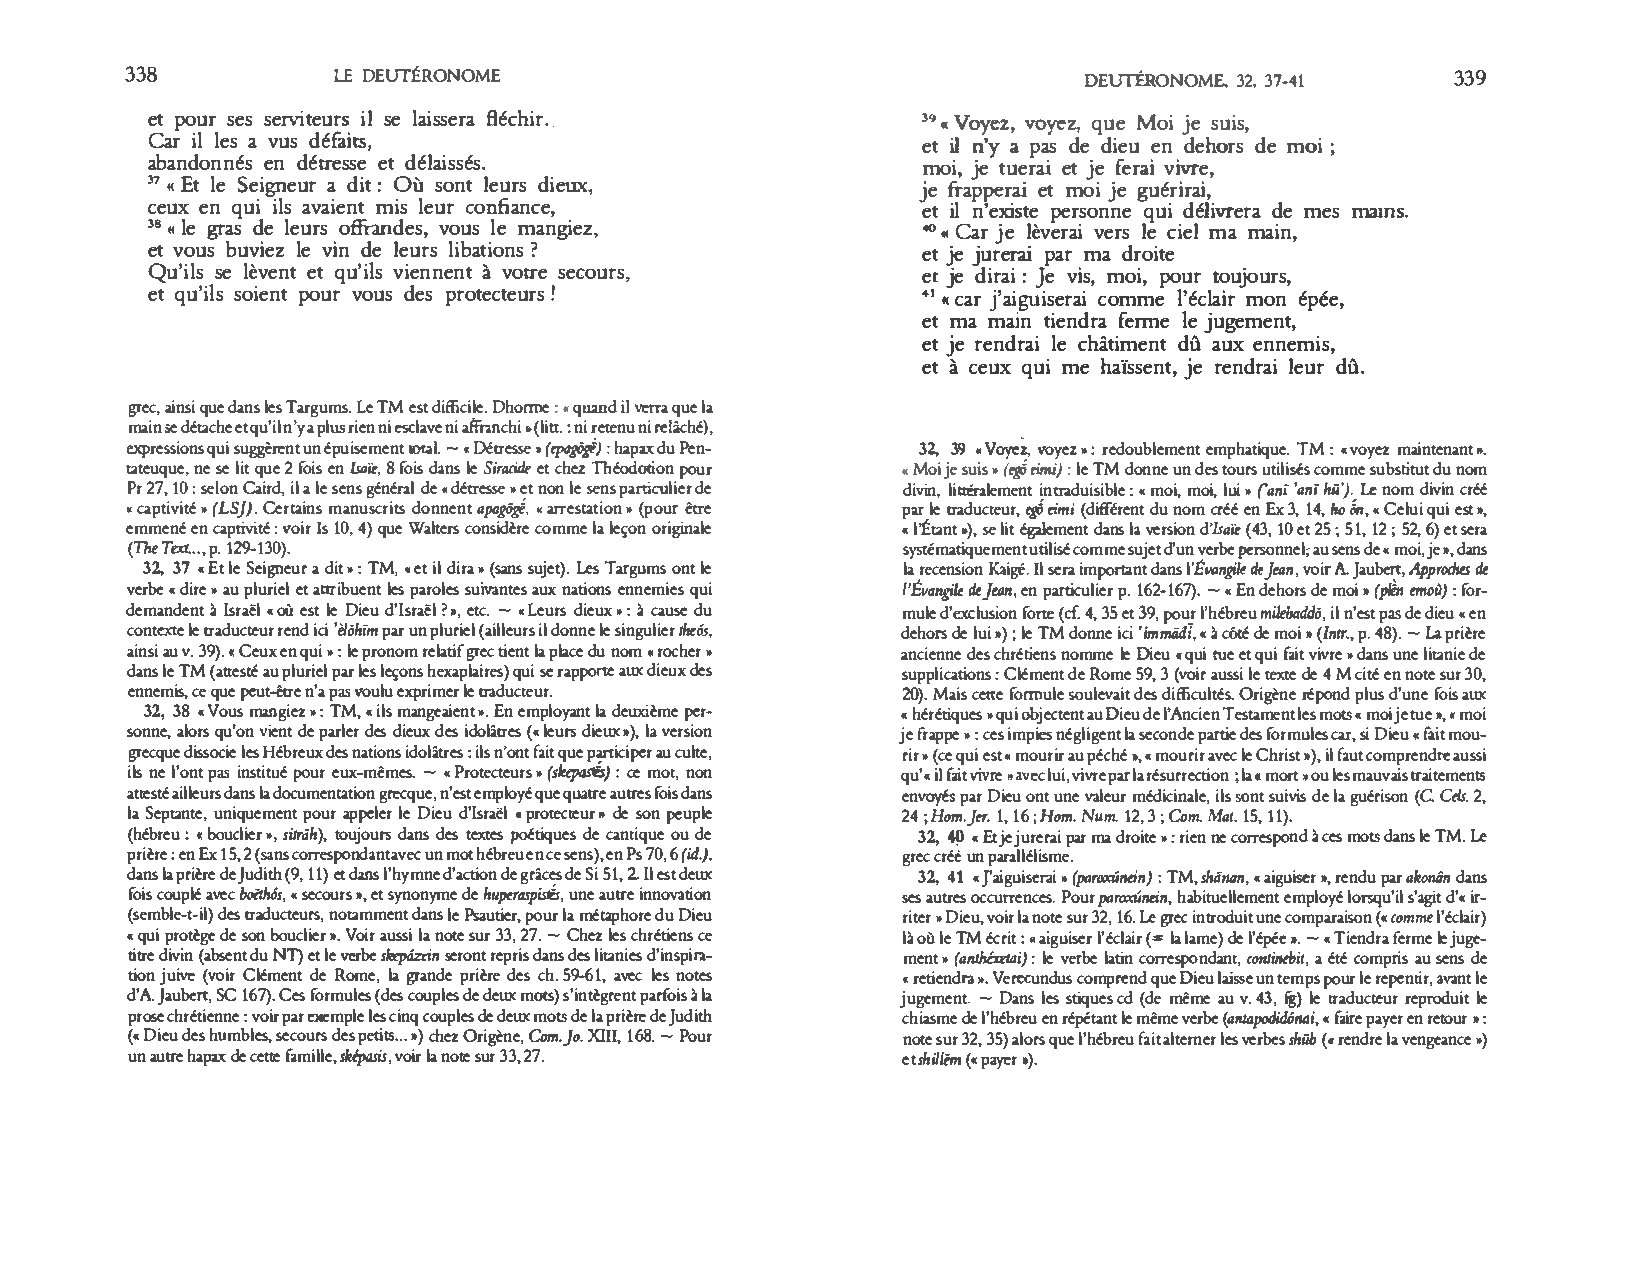
\includepdf[pages=1, angle=90]{img/4Q44/LXX_french.pdf}

\section*{Annexe - Ruth - Edition de Göttingen - Udo Quast}

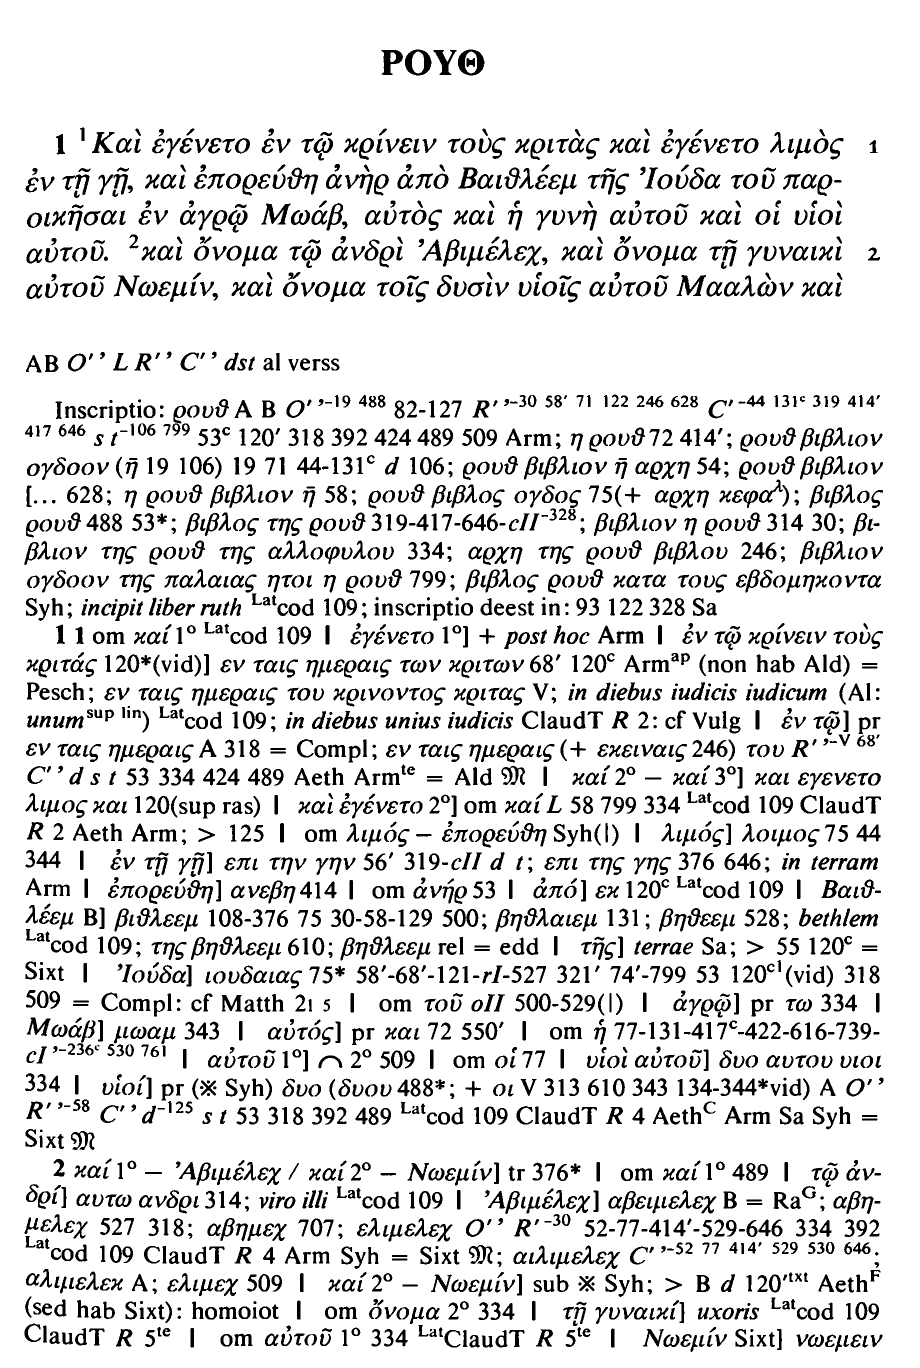
\includegraphics[width=\textwidth]{img/LXX_ruth_1_1.png}
\newpage
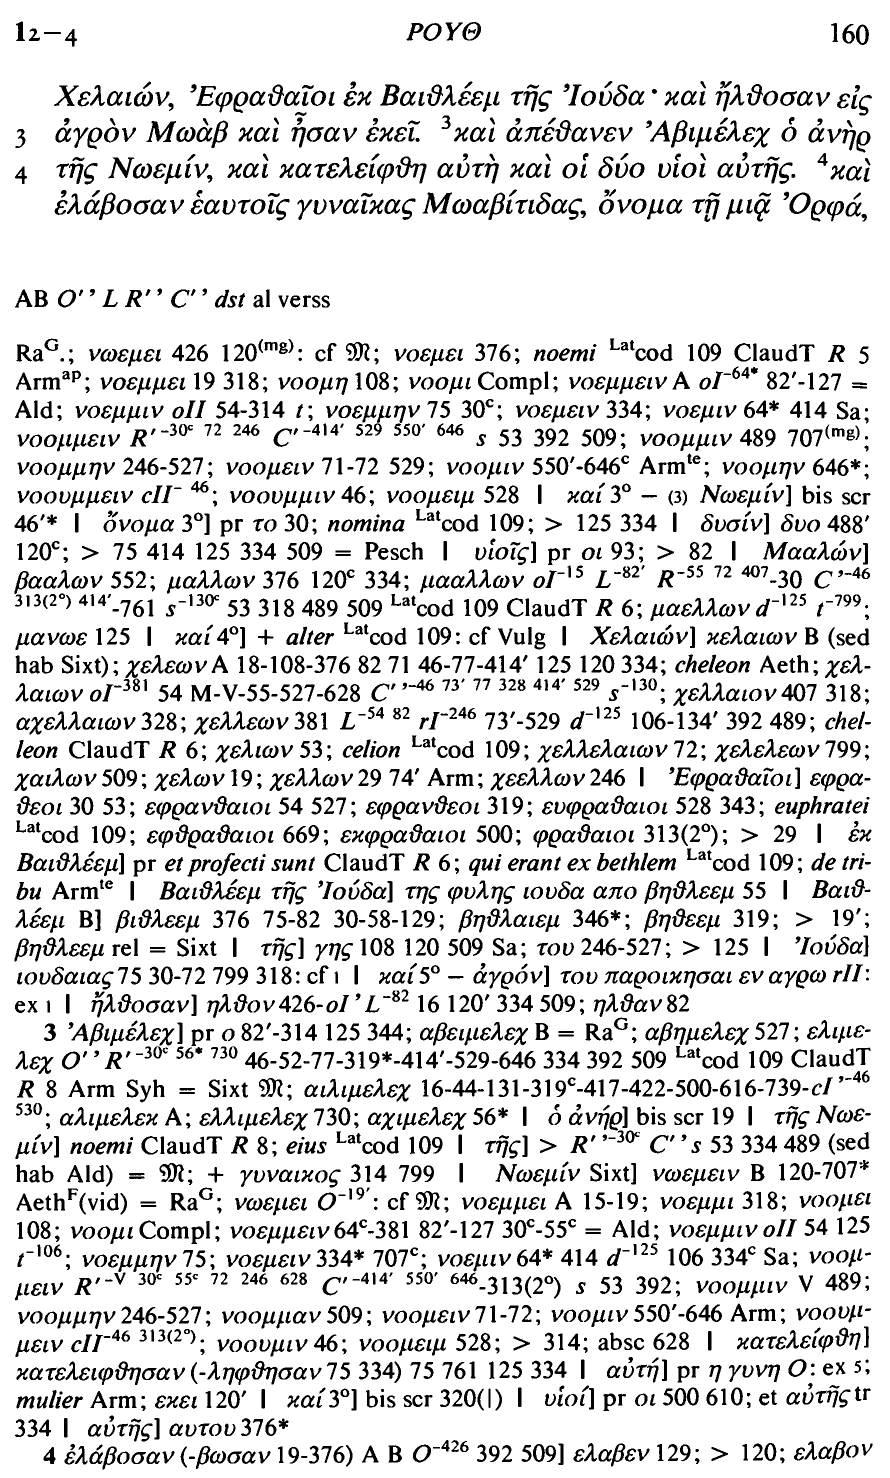
\includegraphics[width=\textwidth]{img/LXX_ruth_1_2.png}

\section*{Annexe  - Ruth (Codex Alexandrinus)}
    Source : \href{https://manuscripts.csntm.org/Manuscript/Group/GA_02?sequence=999}{https://manuscripts.csntm.org/Manuscript/Group/GA\_02?sequence=999}\\
    
     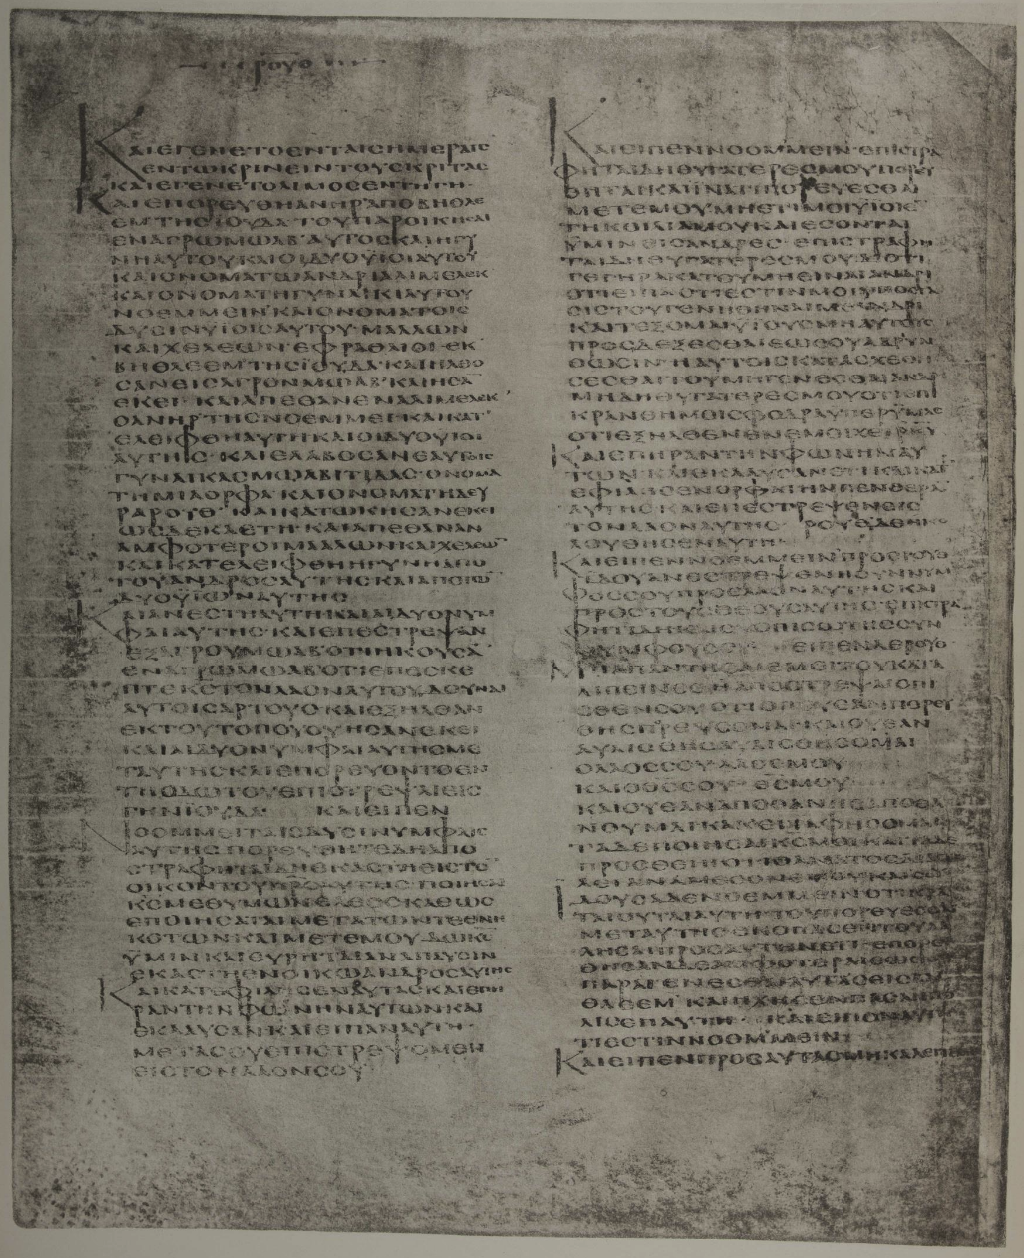
\includegraphics[width=\textwidth]{img/Codex_Alexandrinus_GA02_Ruth_folio_158.png}
     \caption{Codex Alexandrinus - British Library, Royal MS 1 D V, folio 158}
    \newpage

\section*{Annexe - Ruth (Codex Vaticanus Vat.gr. 1209)}
    \Source: \href{https://digi.vatlib.it/view/MSS_Vat.gr.1209}{https://digi.vatlib.it/view/MSS\_Vat.gr.1209}\\
    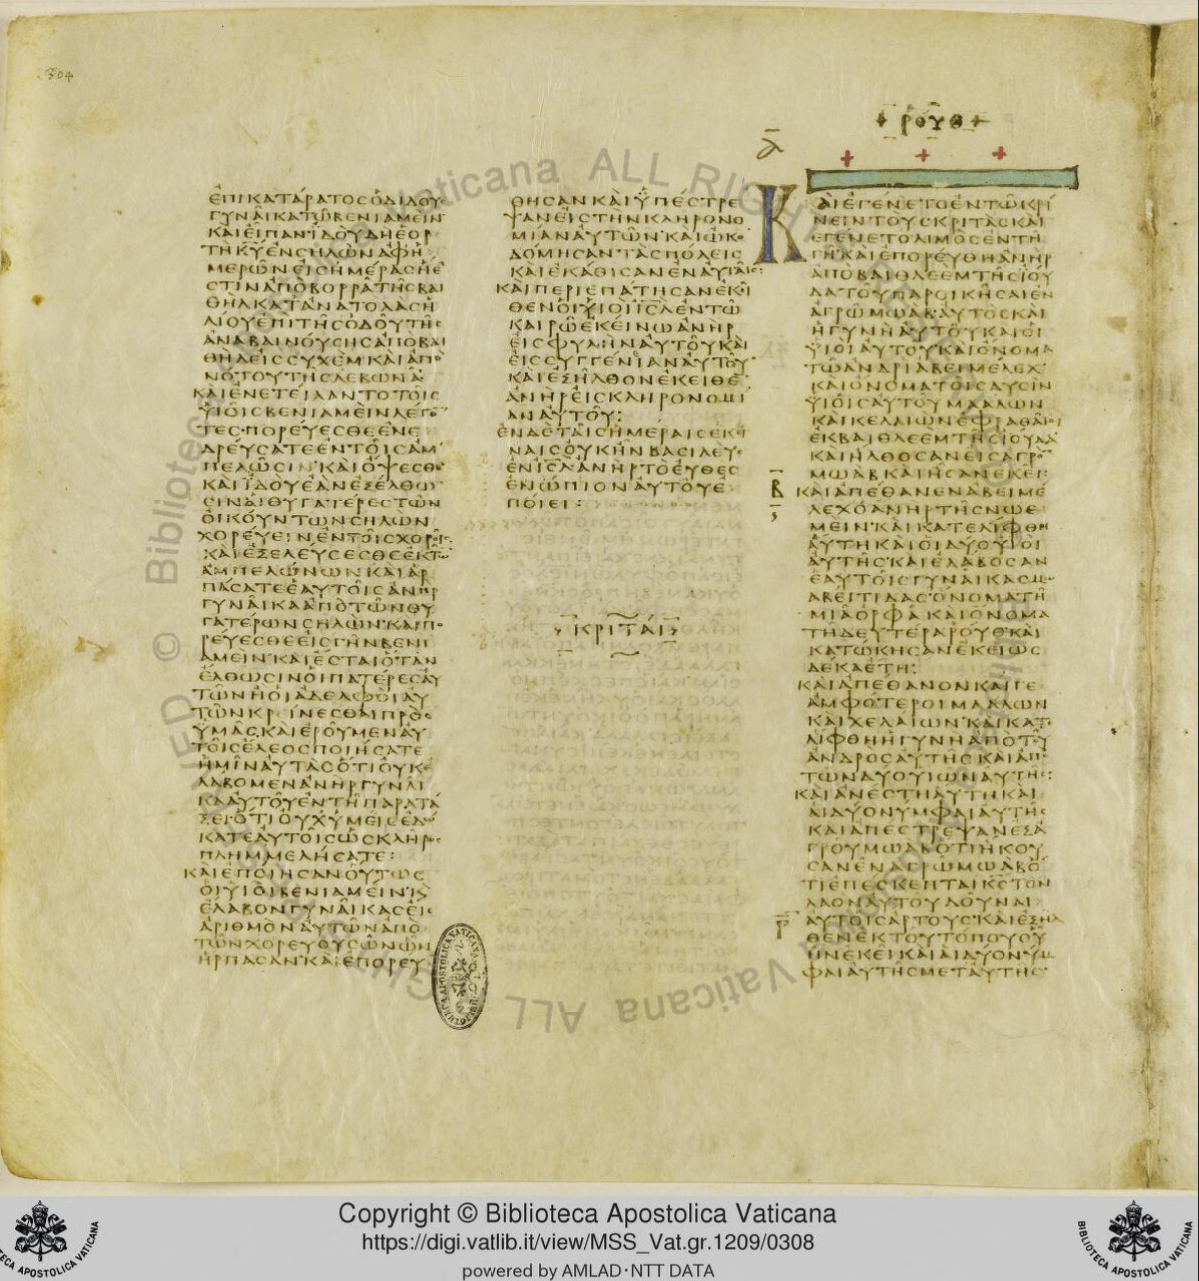
\includegraphics[width=\textwidth]{img/Codex Vaticanus_GA03_Vat.gr1209_fol_304.png}
    \caption{Codex Vaticanus, Bibliothèque du Vatican, Vat.gr. 1209, folio 304}
\end{document}